\section{Einführung}
Abhängig vom Bauteil können Stromstärke und Spannung in verschiedensten Verhältnissen stehen. Diese Verhältnisse werden Grafisch dargestellt als Kennlinien bezeichnet. 
\subsection{Warm- und Kaltleiter}
Aus dem Ohmschen Gesetz ist ein einfaches Verhältnis zwischen Spannung und Stromstärke bekannt. Die Spannung $ U $ ist direkt proportional zur Stromstärke $ I $, wobei der Widerstand $ R $ einen Proportionalitätskoeffizienten darstellt 
\begin{equation}
	U = R\cdot I
\end{equation}
Bei einem idealen ohmschen Widerstand steigt somit die Spannung linear mit der Stromstärke. Der elektrische Widerstand lässt sich aus dem spezifischen elektrischen Widerstand $ \rho $ und der Geometrie des Leiters errechnen. Für homogene Leiter gilt
\begin{equation}
	R = \rho\int\nolimits_l\frac{\mathrm dr}{A(r)} 
\end{equation}
Analog dazu sind elektrischer Leitwert der Kehrwert des elektrischen Widerstandes und spezifische elektrische Leitfähigkeit der Kehrwert des spezifischen elektrischen Widerstandes.  \\
Der spezifische elektrische Widerstand ist material- und temperaturabhängig. Für kleine Temperaturdifferenzen in der Größenordnung von $ \SI{100}{\kelvin} $ verhält sich der spezifische elektrische Widerstand linear zur Temperatur $ T $
\begin{equation}
	\rho = \rho_0 [1 + \alpha(T - T_0)]
\end{equation}
Dabei ist $ \rho_0 $ der spezifische Widerstand bei der Temperatur $ T_0 $ und $ \alpha $ Proportionalitätskonstante. Entsprechend ist $ \alpha $ gegeben durch
\begin{equation}
	\alpha = \frac{1}{\rho_0} \frac{\Delta \rho}{\Delta T}
\end{equation}
In jedem realen Leiter wird durch den Stromfluss eine Verlustleistung erzeugt, die den Leiter erwärmt. Dieses Prinzip ist insbesondere bei einer Glühlampe zu beobachten. Der Draht wird fängt durch den Stromfluss an zu glühen und emittiert dadurch Licht. Da sich mit der Zunahme der Temperatur der spezifische elektrische Widerstand ändert ist die $ I $-$ U $-Kurve nicht linear. Bei Warmleitern wie Metallen flacht die Kurve mit zunehmender Spannung ab, bei Kaltleitern dagegen wird die Kurve zunehmend steiler.

\subsection{Halbleiter}
Halbleiter zeichnen sich dadurch aus, dass für kleine Spannungen der Strom bevorzugt in eine Richtung fließt. Meistens werden dazu heutzutage Grenzschichten aus n-dotierten und p-dotierten Silizium verwenden. Dabei besitzt das n-Dotierte Silizium durch ein eingearbeitetes Element aus der fünften Hauptgruppe freie negative Ladung, während das p-dotierte Silizium durch ein Element der dritten Hauptgruppe freie positive Ladung besitzt. An der Grenzschicht diffundieren die freien negativen Ladungen in die p-Schicht und es wird ein Elektrisches Feld mit negativem Pol an der p-Schicht erzeugt. Dieses Feld wird Raumladungszone genannt. Durch den Ladungsübergang in die p-Schicht existieren hier weniger freie Ladungen und somit nimmt der Widerstand zu. Legt man den positiven Pol der äußeren Spannung an der p-Schicht an, so wirkt man dem elektrischen Feld entgegen und in der Raumladungszone sind mehr freie Ladungen, so dass die Leitfähigkeit zunimmt. Legt man die Spannung entgegengesetzt an, so wird die Raumladungszone entsprechend vergrößert und der Widerstand bleibt groß. Ab einer gewissen, von der jeweiligen Diode abhängigen, Durchbruchspannung nimmt der Widerstand rapide ab. Dabei werden normale Dioden nachhaltig geschädigt, während Z-Dioden auf diesen Betrieb ausgelegt sind und so zur Spannungsregulierung verwendet werden können.

\subsection{Glimmlampe}
Bei der Glimmlampe werden zwischen einer Kathode und einer Anode eine Spannung angelegt. Ist diese Spannung zu klein, kann kein Strom fließen. Ab der Zündspannung kommt es zum Überschlag, so dass das enthaltene Gas ionisiert wird. Durch die Ionisierung kann nun auch bei geringerer Spannung Strom fließen, bis die Löschspannung unterschritten wird. Das Ionisierte Gas emittiert bei der Entladung elektromagnetische Wellen. Je nach Gas können diese im Bereich des sichtbaren Lichts liegen. 

\section{Versuch}
Im Folgendem werden die Kennlienen von verschieden Bauteilen mit dem Aufbau~\ref{fig:aufbau} bestimmt. Die Messfehler für Strom und Spannung variierten aufgrund von Skalenwechseln am Multimeter auch innerhalb einer Messreihe. Im Einzelnen sind sie im Laborbuch vermerkt.
\begin{figure}[H]
	\centering
	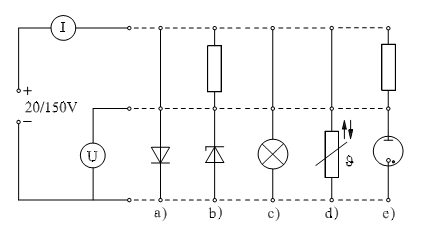
\includegraphics[width=.8\textwidth]{Aufbau.png}
	\caption{Messaufbau für unterschiedliche Leiter}
	\label{fig:aufbau}
\end{figure}
\subsection{Diode in Durchlassrichtung}
Wie in Abbildung~\ref{fig:aufbau} a) gezeigt wird der Strom für unterschiedliche Spannung gemessen, um daraus eine U-I-Kennlinie zu ermitteln.

\begin{figure}[H]
\centering
\begin{tikzpicture}
  \begin{axis}[
    width=15 cm,
    height=9 cm,
    xmin=0, xmax=0.8,
    ymin=-1, ymax=60,
    xlabel={$U$ [\si{mV}]},
    ylabel={$I$ [\si{mA}]},
    domain=0:0.8,
    cycle list name=color list,
    legend entries={Messwerte, $a\cdot b^x$},
    legend pos=north west
  ]
  \addplot+ plot [only marks,mark=x, error bars/.cd, x dir=both, x fixed=0.002, y dir=both, y explicit]  table[y error index=2] {Diode.txt};
  \addplot+ plot [samples=200, mark=none] {5.61784*10^(-7)*(1.69598*10^11)^x};
  \end{axis}
\end{tikzpicture}
\caption{Messwerte und Fit für eine Diode in Durchlassrichtung}
\label{fig:diode}
\end{figure}
Die Fehlerbalken sind sehr kurz und deshalb schwer zu erkennen.

Aufgrund des anscheinend exponentiellen Verlaufs der Messwerte wurde mit \emph{gnuplot} nach dem \emph{least-squares}-Verfahren die Werte gegen die Funktion $f(x)=a\cdot b^x$ gefittet. Ausgabe:
\begin{table}[H]
  \centering
  \begin{tabular}{c | c | c }
    Variable  & Wert & Unsicherheit\\ \hline
    a & $\num{5.61784d-7}$ & $\pm\num{3.084d-8}$ \\
    b & $\num{1.69598d+11}$ & $\pm\num{1.319d+10}$
  \end{tabular}
  \caption{Linearer Fit zu Abbildung~\ref{fig:diode}}
  \label{tab:fitdiode}
\end{table}
\subsection{Zenerdiode}
Wie in Abbildung~\ref{fig:aufbau} b) gezeigt wird der Strom für unterschiedliche Spannung gemessen, um daraus eine U-I-Kennlinie zu ermitteln. Dies wird jedoch einmal mit einer Polung in Durchlassrichtung und einmal in Sperrrichtung getan.
\begin{figure}[H]
\centering
\begin{tikzpicture}
  \begin{axis}[
    width=15 cm,
    height=9 cm,
    xmin=0, xmax=6,
    ymin=-1, ymax=30,
    xlabel={$U$ [\si{V}]},
    ylabel={$I$ [\si{mA}]},
    domain=0:6,
    cycle list name=color list,
    legend entries={Messwerte, $a\cdot b^x$},
    legend pos=north west
  ]
  \addplot+ plot [only marks,mark=x, error bars/.cd, x dir=both, x fixed=0.002, y dir=both, y explicit]  table[y error index=2] {Diodesperr.txt};
  \addplot+ plot [samples=200, mark=none] {1.50271*10^(-7)*(42.7533)^x};
  \end{axis}
\end{tikzpicture}
\caption{Messwerte und Fit für eine Zenerdiode in Sperrrichtung}
\label{fig:diodesperr}
\end{figure}
Die Fehlerbalken sind sehr kurz und deshalb schwer zu erkennen.

Aufgrund des anscheinend exponentiellen Verlaufs der Messwerte wurde mit \emph{gnuplot} nach dem \emph{least-squares}-Verfahren die Werte gegen die Funktion $f(x)=a\cdot b^x$ gefittet. Ausgabe:
\begin{table}[H]
  \centering
  \begin{tabular}{c | c | c }
    Variable & Wert & Unsicherheit\\ \hline
    a & $\num{1.50271d-7}$ & $\pm\num{5.433d-8}$ \\
    b & $\num{42.7533}$ & $\pm\num{3.073}$
  \end{tabular}
  \caption{Linearer Fit zu Abbildung~\ref{fig:diodesperr}}
  \label{tab:fitdiodesperr}
\end{table}
\begin{figure}[H]
\centering
\begin{tikzpicture}
  \begin{axis}[
    width=15 cm,
    height=9 cm,
    xmin=0, xmax=0.8,
    ymin=-1, ymax=40,
    xlabel={$U$ [\si{V}]},
    ylabel={$I$ [\si{mA}]},
    domain=0:0.8,
    cycle list name=color list,
    legend entries={Messwerte, $a\cdot b^x$},
    legend pos=north west
  ]
  \addplot+ plot [only marks,mark=x, error bars/.cd, x dir=both, x fixed=0.002, y dir=both, y explicit]  table[y error index=2] {Diodedurch.txt};
  \addplot+ plot [samples=200, mark=none] {3.08803*10^(-11)*(9.72068*10^16)^x};
  \end{axis}
\end{tikzpicture}
\caption{Messwerte und Fit für eine Zenerdiode in Durchlassrichtung}
\label{fig:diodedurch}
\end{figure}
Die Fehlerbalken sind sehr kurz und deshalb schwer zu erkennen.

Aufgrund des anscheinend exponentiellen Verlaufs der Messwerte wurde mit \emph{gnuplot} nach dem \emph{least-squares}-Verfahren die Werte gegen die Funktion $f(x)=a\cdot b^x$ gefittet. Ausgabe:
\begin{table}[H]
  \centering
  \begin{tabular}{c | c | c }
    Variable & Wert & Unsicherheit\\ \hline
    a & $\num{3.08803d-11}$ & $\pm\num{3.759d-12}$ \\
    b & $\num{9,72068d16}$ & $\pm\num{1.673d16}$
  \end{tabular}
  \caption{Linearer Fit zu Abbildung~\ref{fig:diodedurch}}
  \label{tab:fitdiodedurch}
\end{table}
\subsection{Glühlampe}
Wie in Abbildung~\ref{fig:aufbau} c) gezeigt wird der Strom für unterschiedliche Spannung gemessen, um daraus eine U-I-Kennlinie zu ermitteln.

\begin{figure}[H]
\centering
\begin{tikzpicture}
  \begin{axis}[
    width=15 cm,
    height=9 cm,
    xmin=0, xmax=14,
    ymin=0, ymax=60,
    xlabel={$U$ [\si{V}]},
    ylabel={$I$ [\si{mA}]},
    domain=0:14,
    cycle list name=color list,
    legend entries={Messwerte, $a\sqrt{x}$},
    legend pos=north west
  ]
  \addplot+ plot [only marks,mark=x, error bars/.cd, x dir=both, x fixed=0.002, y dir=both, y explicit]  table[y error index=2] {Lampe.txt};
  \addplot+ plot [samples=200, mark=none] {14.9315*sqrt(x)};
  \end{axis}
\end{tikzpicture}
\caption{Messwerte und Fit für eine Lampe}
\label{fig:Lampe}
\end{figure}
Die Fehlerbalken sind sehr kurz und deshalb schwer zu erkennen.

Aufgrund des anscheinend Wurzel-artigem Verlaufs der Messwerte, besonders im Bereich bis $3V$, wurde mit \emph{gnuplot} nach dem \emph{least-squares}-Verfahren die Werte gegen die Funktion $f(x)=a\cdot\sqrt{x}$ gefittet. Ausgabe:
\begin{table}[H]
  \centering
  \begin{tabular}{c | c | c }
    Variable & Wert & Unsicherheit\\ \hline
    a & $\num{14,9315}$ & $\pm\num{0,2092}$ \\
   
  \end{tabular}
  \caption{Linearer Fit zu Abbildung~\ref{fig:Lampe}}
  \label{tab:fitlampe}
\end{table}
\subsection{NTC}
Wie in Abbildung~\ref{fig:aufbau} d) gezeigt wird der Strom für unterschiedliche Spannung gemessen, um daraus eine U-I-Kennlinie zu ermitteln. Dabei muss nach jeder Spannungserhöhung gewartet werden, bis sich der Temperaturgradient abgebaut hat. 

\begin{figure}[H]
\centering
\begin{tikzpicture}
  \begin{axis}[
    width=15 cm,
    height=9 cm,
    xmin=0, xmax=8,
    ymin=0, ymax=60,
    xlabel={$U$ [\si{V}]},
    ylabel={$I$ [\si{mA}]},
    domain=0:8,
    cycle list name=color list,
    legend entries={Messwerte, $ax^2+bx+c$},
    legend pos=north west
  ]
  \addplot+ plot [only marks,mark=x, error bars/.cd, x dir=both, x fixed=0.01, y dir=both, y explicit]  table[y error index=2] {NTC1.txt};
  \addplot+ plot [samples=200, mark=none] {0.316693*x^2-0.0533435*x+1.05214};
  \end{axis}
\end{tikzpicture}
\caption{Messwerte und Fit für eine NTC-Widerstand}
\label{fig:ntc}
\end{figure}
Die Fehlerbalken sind sehr kurz und deshalb schwer zu erkennen.

Aufgrund des anscheinend quadratischem Verlaufs der Messwerte wurde mit \emph{gnuplot} nach dem \emph{least-squares}-Verfahren die Werte gegen die Funktion $f(x)=a\cdot x^2+b\cdot x+c$ gefittet. Beim Fitten wurde der letzte Messwert nicht betrachtet, da er vollkommen aus dem Verlauf der Werte herausfällt. Dies ist auf ein Versagen der Leistung des Netzgeräts zurückzuführen. Ausgabe:
\begin{table}[H]
  \centering
  \begin{tabular}{c | c | c }
    Variable   & Wert & Unsicherheit\\ \hline
    a & $\num{0,316693}$ & $\pm\num{0,05691}$ \\
    b & $\num{-0,0533435}$ & $\pm\num{0,4446}$ \\
    c & $\num{1,05214}$ & $\pm\num{0,6146}$ \\
  \end{tabular}
  \caption{Quadratischer Fit zu Abbildung~\ref{fig:ntc}}
  \label{tab:fitntc}
\end{table}
\subsection{Glimmlampe}
Wie in Abbildung~\ref{fig:aufbau} e) gezeigt wird der Strom für unterschiedliche Spannnungen gemessen. Dabei wird zuerst durch langsames Hochdrehen der Spannung bis zur Zündung der Lampe die Zündspannung bestimmt. Anschließend wird die Spannung langsam reduziert, bis die Glimmlampe erlischt, um die Löschspannung zu bestimmen. Wir erhalten als Mittelwerte für jeweils drei Messungen:
\begin{table}[H]
  \centering
  \begin{tabular}{c | c}
    Zündspannung & \SI{112.0(1)}{V} \\ \hline
    Löschspannung & \SI{83.3(1)}{V} \\
  \end{tabular}
  \caption{Messergebnis zur Glimmlampe}
  \label{tab:glimm}
\end{table}

Anschließend messen wir den Strom von der höchstmöglichen bis zur Löschspannung durch:

\begin{figure}[H]
\centering
\begin{tikzpicture}
  \begin{axis}[
    width=15 cm,
    height=9 cm,
    xmin=83.2, xmax=86.9,
    ymin=1.2, ymax=15.8,
    xlabel={$U$ [\si{V}]},
    ylabel={$I$ [\si{mA}]},
    domain=83.2:86.9,
    cycle list name=color list,
    legend entries={Messwerte, $ax+b$},
    legend pos=north west
  ]
  \addplot+ plot [only marks,mark=x, error bars/.cd, x dir=both, x fixed=0.1, y dir=both, y fixed=0.02]  table {glimm.txt};
  \addplot+ plot [mark=none] {3.93146*x-325.67};
  \end{axis}
\end{tikzpicture}
\caption{Messwerte für die Glimmlampe}
\label{fig:glimm}
\end{figure}
Aufgrund des anscheinend linearen Verlaufs der Messwerte wurde mit \emph{gnuplot} nach dem \emph{least-squares}-Verfahren die Werte gegen die Funktion $f(x)=a\cdot x +b$ gefittet. Ausgabe:
\begin{table}[H]
  \centering
  \begin{tabular}{c | c | c }
    Variable   & Wert & Unsicherheit\\ \hline
    a & $\num{3.93146}$ & $\pm\num{0.07344}$ \\
    b & $\num{-325.67}$ & $\pm\num{6.243}$ \\
  \end{tabular}
  \caption{Linearer Fit zu Abbildung \ref{fig:glimm}}
  \label{tab:fitglimm}
\end{table}
\subsection{Temperaturabhängigkeit des Widerstandes eines Metalldrahtes}
Der Zusammenhang aus der Theorie gilt für den spezifischen Widerstand $\rho$, jedoch messen wir im Versuch den Widerstand $R=\rho\cdot l/A$, wobei $l$ die Länge des Leiters und $A$ die Querschnittsfläche ist. Wir gehen näherungsweise davon aus, dass die thermische Ausdehnung während des Versuches gering ist und nehmen deshalb $l$ und $A$ als konstant an. Für den Fit definieren wir $C\coloneqq \rho_0\cdot l/A$.

Die Messwerte werden für Aufheizen bzw. Abkühlen getrennt mit \emph{gnuplot} nach dem \emph{least-squares}-Verfahren gegen die aus der Theorie erwartete Funktion $R(T)=C(1+\alpha\cdot T$ gefittet. 
\begin{figure}[H]
\centering
\begin{tikzpicture}
  \begin{axis}[
    width=15 cm,
    height=9 cm,
    xmin=22, xmax=90,
    ymin=5.5, ymax=7,
    xlabel={$T$ [\si{\degreeCelsius}]},
    ylabel={$R$ [\si{\ohm}]},
    domain=22:90,
    cycle list name=color list,
    legend entries={Messwerte, $C_{\text{auf}}(1+\alpha_{\text{auf}}\cdot T)$},
    legend pos=north west
  ]
  \addplot+ plot [only marks,mark=x, error bars/.cd, x dir=both, x fixed=2, y dir=both, y fixed=0.126]  table {aufheizen.txt};
  \addplot+ plot [mark=none] {5.06455*(1+0.00448047*x)};
  \end{axis}
\end{tikzpicture}
\caption{Messwerte und Fit fürs Aufheizen}
\label{fig:aufheizen}
\end{figure}

\begin{table}[H]
  \centering
  \begin{tabular}{c | c}
    Variable & Wert \\ \hline
    $C_{\text{auf}}$ & $\SI{5.06455(3523)}{\ohm}$ \\
    $\alpha_{\text{auf}}$ & $\SI{4.48047(16030)}{\milli\ohm\per\degreeCelsius}$ \\
  \end{tabular}
  \caption{Fit zu Abbildung~\ref{fig:aufheizen}}
  \label{tab:fitaufheizen}
\end{table}
\begin{figure}[H]
\centering
\begin{tikzpicture}
  \begin{axis}[
    width=15 cm,
    height=9 cm,
    xmin=24, xmax=89,
    ymin=5.5, ymax=7,
    xlabel={$T$ [\si{\degreeCelsius}]},
    ylabel={$R$ [\si{\ohm}]},
    domain=24:87,
    cycle list name=color list,
    legend entries={Messwerte, $C_{\text{ab}}(1+\alpha_{\text{ab}}\cdot T)$},
    legend pos=north west
  ]
  \addplot+ plot [only marks,mark=x, error bars/.cd, x dir=both, x fixed=2, y dir=both, y fixed=0.126]  table {abkuehlen.txt};
  \addplot+ plot [mark=none] {5.06929*(1+0.00430956*x)};
  \end{axis}
\end{tikzpicture}
\caption{Messwerte und Fit fürs Abkühlen}
\label{fig:abkuehlen}
\end{figure}
\begin{table}[H]
  \centering
  \begin{tabular}{c | c}
    Variable & Wert \\ \hline
    $C_{\text{ab}}$ & $\SI{5.06929(2510)}{\ohm}$ \\
    $\alpha_{\text{ab}}$ & $\SI{4.30956(10240)}{\milli\ohm\per\degreeCelsius}$ \\
  \end{tabular}
  \caption{Fit zu Abbildung~\ref{fig:abkuehlen}}
  \label{tab:fitabkuehlen}
\end{table}
\section{Diskussion}


\subsection{Temperaturabhängigkeit des Widerstandes eines Metalldrahtes}
Bei der Untersuchung der Temperaturabhängigkeit des Widerstandes eines Drahtes hat sich bei unserer Messreihe gezeigt, dass die lineare Näherung in Rahmen unserer Messgenauigkeit völlig ausreicht. Zudem ist zu beobachten, dass im Abweichung bei erwärmen und abkühlen im Rahmen der Unsicherheit liegt und somit von einem reversiblen Prozess ausgegangen werden kann. Bei der Versuchsdurchführung war es insbesondere schwierig, die Temperatur genau zu bestimmen. Sowohl bei dem Erwärmen als auch beim Abkühlen war keine homogene Temperaturverteilung zu beobachten. Je nach Positionierung des Thermometers konnte die gemessene Temperatur deutlich schwanken. Da das Abkühlen deutlich langsamer statt fand, als das erwärmen, kann man hier von einer besseren Temperaturverteilung ausgehen. Zudem liegen die Messwerte beim Abkühlen genauer auf der Ausgleichsgeraden. Somit stimmt beim Abkühlen sowohl die Durchführung besser mit der optimalen Durchführung überein als auch das Resultat mit der Theorie. Wollte man maximale Genauigkeit bei der Temperatur erreichen, müsste man das Wärmebad langsam erhitzen und bevor man den Messwert nimmt eine Zeit lang auf der gleichen Temperatur halten, bis diese sich homogen verteilt hat. Dies wäre aber im Rahmen des Praktikums zu aufwändig. 
\notecite{anleitung-ws2014}
